\linespread{1.5}
%use \usepackage{float}
\textbf{Solução}

\textbf{a)}
Por estar usando a ferramenta computacional \textit{https://www.desmos.com/calculator} foi necessário escolher um valor para \textit{T} a fim de criar a imagem do gráfico abaixo. Para esse exemplo, foi escolhido $T = 5$.

\begin{figure}[H]
    \centering
    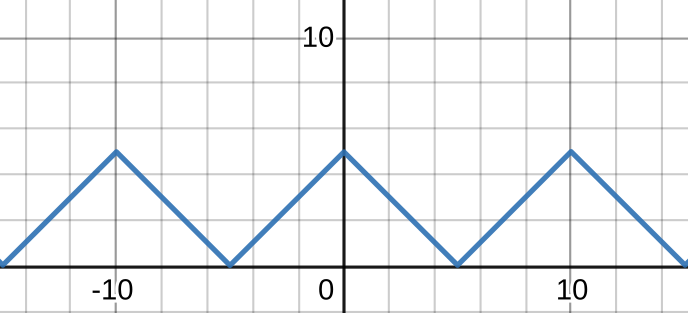
\includegraphics[width=0.5\linewidth]{fig/sf5a.png}
\end{figure}

\textbf{b)}

Analisando o gráfico acima podemos ver por sua simetria que a função é uma função par.

\textbf{c)}
Dada a equação que define a série de Fourier real:
\begin{equation}
    \label{eq:Fourierserie}
    f(t) = a_0 + \sum_{k=1}^\infty a_k\cos{(kwt)} + b_k\sin{(kwt)}
\end{equation}

Como $f(x)$ é par, não se faz necessário calcular $b_k$ pois:
\begin{equation}
    \label{eq:sf5cbk}
    b_k = 0
\end{equation}

\begin{equation*}
    a_0 = \frac{1}{2T}\left[\int_{-T}^0 (T+x)dx + \int_0^T (T-x)dx \right] = \frac{1}{2T}\left[\left(Tx + \frac{x^2}{2}\right)^0_{-T} + \left[Tx - \frac{x^2}{2}\right)^T_0\right] 
\end{equation*}
\begin{equation*}
    a_0 = \frac{1}{2T}\left[-\left(-T^2 + \frac{T^2}{2}\right) + \left(T^2 - \frac{T^2}{2}\right)\right] = \frac{1}{2T}\left(\frac{T^2}{2} + \frac{T^2}{2}\right) 
\end{equation*}
\begin{equation}
    \label{eq:sf5ca0}
    a_0 = \frac{T}{2}
\end{equation}

\begin{equation*}
    a_k = \frac{1}{T}\left[\int_{-T}^0 (T+x)\cos{(kwx)}dx +  \int_0^T (T-x)\cos{(kwx)}dx \right]
\end{equation*}
\begin{equation*}
    a_k = \frac{1}{T}\left[\int_{-T}^0 (T\cos{(kwx)} + x\cos{(kwx)})dx + \int_0^T (T\cos{(kwx)} - x\cos{(kwx)})dx \right]
\end{equation*}
\begin{equation*}
    a_k = \frac{1}{T}\left(\int_{-T}^0 T\cos{(kwx)}dx + \int_{-T}^0 x\cos{(kwx)}dx + \int_0^T T\cos{(kwx)}dx - \int_0^T T -x\cos{(kwx)}dx \right)
\end{equation*}
\begin{equation*}
    a_k = \frac{1}{T}((I) + (II) + (III) + (IV)) 
\end{equation*}

Sabendo que $w = \frac{2\pi}{Per} = \frac{2\pi}{2T} = \frac{\pi}{T}$, então:

\begin{equation*}
    (I) = \int_{-T}^0 T\cos{(kwx)}dx = \left[\frac{T}{kw}\sin{(kwx)}\right]^0_{-T} = \left[\frac{T}{kw}\sin{0}- \frac{T}{kw}\sin{(-kwT)}\right]
\end{equation*}
\begin{equation}
    \label{eq:sf5cI}
    (I) = \frac{T\sin{(kwT)}}{kw} = \frac{T^2\sin{(k\pi)}}{k\pi}
\end{equation}
Como $\forall \hspace{1mm} k\in\N$ e para $k\geq1$, $\sin{k\pi} = 0$. Logo $(I) =0$

Para o $(II)$ devemos resolver a integral, por partes:
\begin{equation*}
    (II) = \int_{-T}^0 x\cos{(kwx)}dx = \left[\frac{x\sin{(kwx)}}{kw}\right]^0_{-1} - \int_{-T}^0\frac{\sin(kwx)}{kw}dx
\end{equation*}
\begin{equation*}
    = \left[\frac{x\sin{(kwx)}}{kw}\right]^0_{-T} - \left[-\frac{\cos{(kwx)}}{(kw)^2}\right]^0_{-T} = \left(\frac{T\sin{(-kwT)}}{kw}\right) - \left[-\frac{cos0}{(kw)^2} - \left(-\frac{\cos{(-kwT)}}{(kw)^2}\right)\right]
\end{equation*}
com a função seno sendo impar e a função cosseno sendo par, temos:
\begin{equation*}
    =\left(-\frac{T\sin{(kwt)}}{kw}\right)-\left[\left(-\frac{1}{(kw)^2} + \frac{\cos{kwT}}{(kw)^2}\right)\right]
\end{equation*}
substituindo $w = \frac{\pi}{T}$ temos então:
\begin{equation*}
    -\frac{T^2\sin{(k\pi)}}{k\pi} + \frac{T^2}{(k\pi)^2} - \frac{T^2\cos{k\pi}}{(k\pi)^2}
\end{equation*}
Sabemos que $\sin{(k\pi)} = 0 \forall k \in \Z$, portanto:
\begin{equation}
    \label{eq:sf5cIIns}
    (II) = \frac{T^2}{(k\pi)^2}(1 - \cos{(k\pi)}
\end{equation}
Se analisarmos essa equação, vemos que $1- \cos{(k\pi)} = 0$, quando $\cos{(k\pi)} = 1$ e isso só ocorre para $k$ par. Para $k$ ímpar, $1- \cos{(k\pi)} = 2$. Portanto a equação anterior pode ser reescrita da seguinte forma:
\begin{equation}
    \label{eq:sf5cIIs}
    (II) = \frac{2T^2}{(2k-1)^2\pi^2}
\end{equation}

Agora resolvemos $(III)$:
\begin{equation*}
    (III) = \int^T_0 T\cos{kwx}dx = \left[-\frac{x\sin{(kwx)}}{kw}\right]^T_0 = \frac{T^2\sin{(k\pi)}}{k\pi} = 0\forall k \in \Z
\end{equation*}
Por fim resolvemos $(IV)$, novamente por partes:
\begin{equation*}
    (IV) = \int^T_0 (-x\cos{(kwx)}dx = \left[\frac{-x\sin{(kwx)}}{kw}\right]^T_0 - \int^T_0 -\frac{\sin{(kwx)}}{kw}dx
\end{equation*}
O primeiro item sabemos que é zero já:
\begin{equation*}
    = - \left[\frac{\cos{(kwx)}}{kw}\right]^T_0 = -\left[\frac{\cos{(kwT)}}{(kw)^2} - \frac{1}{(kw)^2}\right]
\end{equation*}
logo:
\begin{equation}
    (IV) = \frac{1}{(kw)^2}(1-\cos{(kwT)}
\end{equation}
Dessa forma $(IV) = (II)$. Subistituindo então $(I), (II), (III), (IV)$ em $a_k$, temos:
\begin{equation}
    a_{2k-1} = \frac{1}{T}\left[\frac{4T^2}{(2k-1)^2\pi^2}\right] = \frac{4T}{(2k-1)^2\pi^2}
\end{equation}
Enfim, a série de Fourier será dada por:
\begin{equation}
    \label{eq:sf5c}
    \boxed{f(x) = \frac{T}{2} + \sum^\infty_{k=1} \frac{4T}{(2k-1)^2\pi^2} \cos{\left[\frac{(2k-1)\pi x}{T}\right]}}
\end{equation}
